\documentclass[12pt, a4paper]{article}


\usepackage[utf8]{inputenc}
\usepackage[T2A]{fontenc}
\usepackage[russian, english]{babel}


\usepackage{amsmath, amssymb, amsthm, mathtools}
\usepackage{physics}
\usepackage{bm}


\usepackage[dvipsnames]{xcolor}
\usepackage{graphicx}
\graphicspath{{img/}}
\usepackage{tikz}
\usepackage{pgfplots}
\pgfplotsset{compat=1.18}


\usepackage{booktabs}
\usepackage{multirow}
\usepackage{array}
\usepackage{longtable}


\usepackage{listings}
\usepackage{lstautogobble}


\usepackage[
  left=2.5cm, right=2.0cm,
  top=2.5cm,  bottom=2.5cm,
  headheight=15pt
]{geometry}


\usepackage{fancyhdr}


\usepackage{float}
\usepackage{caption}
\usepackage{subcaption}
\captionsetup{font=small, labelfont=bf}


\usepackage{enumitem}
% \usepackage{microtype}  % несовместим с кириллическими bitmap-шрифтами
\usepackage{parskip}
\usepackage{titlesec}

\renewcommand{\sectionmark}[1]{\markboth{#1}{}}
\usepackage[
  colorlinks=true,
  linkcolor=MiptBlue,
  citecolor=MiptBlue,
  urlcolor=MiptBlue
]{hyperref}

\definecolor{MiptBlue}{RGB}{0, 82, 155}
\definecolor{MiptDark}{RGB}{30, 30, 50}
\definecolor{MiptAccent}{RGB}{0, 150, 214}
\definecolor{CodeBg}{RGB}{245, 245, 250}
\definecolor{CodeKw}{RGB}{0, 100, 180}
\definecolor{CodeStr}{RGB}{180, 60, 0}
\definecolor{CodeCmt}{RGB}{100, 130, 100}

\pagestyle{fancy}
\fancyhf{}
\fancyhead[L]{\small\textcolor{gray}{\thesection.\ \leftmark}}
\fancyhead[R]{\small\textcolor{gray}{МФТИ, ФПМИ -- 2026}}
\fancyfoot[C]{\thepage}
\renewcommand{\headrulewidth}{0.4pt}

\titleformat{\section}
  {\Large\bfseries\color{MiptBlue}}
  {\thesection.}{0.7em}{}
  [\vspace{-0.3em}\rule{\linewidth}{0.6pt}]

\titleformat{\subsection}
  {\large\bfseries\color{MiptDark}}
  {\thesubsection.}{0.6em}{}

\titleformat{\subsubsection}
  {\normalsize\bfseries\color{MiptDark}}
  {\thesubsubsection.}{0.5em}{}

\renewcommand{\sectionmark}[1]{\markboth{\thesection.\ #1}{}}
\lstset{
  backgroundcolor=\color{CodeBg},
  basicstyle=\ttfamily\small,
  keywordstyle=\bfseries\color{CodeKw},
  stringstyle=\color{CodeStr},
  commentstyle=\itshape\color{CodeCmt},
  numbers=left,
  numberstyle=\tiny\color{gray},
  numbersep=8pt,
  breaklines=true,
  frame=single,
  framerule=0.4pt,
  rulecolor=\color{gray!40},
  tabsize=4,
  autogobble=true,
  showstringspaces=false,
  captionpos=b,
}

\newtheorem{theorem}{Теорема}[section]
\newtheorem{lemma}[theorem]{Лемма}
\newtheorem{proposition}[theorem]{Утверждение}
\newtheorem{corollary}[theorem]{Следствие}
\theoremstyle{definition}
\newtheorem{definition}[theorem]{Определение}
\newtheorem{remark}[theorem]{Замечание}


\newcommand{\TODO}[1]{\textcolor{orange}{\textbf{[TODO: #1]}}}
\newcommand{\REF}{\textcolor{orange}{\textbf{[?]}}}
\newcommand{\N}{\mathbb{N}}
\newcommand{\Z}{\mathbb{Z}}
\newcommand{\Q}{\mathbb{Q}}
\newcommand{\R}{\mathbb{R}}
\newcommand{\CC}{\mathbb{C}}
\newcommand{\F}{\mathbb{F}}
 


\begin{document}



% ============================================================
%  titlepage.tex -- титульный лист + аннотация
% ============================================================

\begin{titlepage}
  \thispagestyle{empty}
  \vspace*{1cm}

  {\color{MiptBlue}\rule{\linewidth}{2pt}}\\[0.5cm]

  \begin{center}
    {\Large\bfseries Московский физико-технический институт}\\[0.2cm]
    {\large Физтех-школа прикладной математики и информатики (ФПМИ)}\\[0.8cm]

    {\huge\bfseries Отчёт по математическому практикуму}\\[0.4cm]
    {\large 1 курс \quad|\quad 2 семестр 2025/26}\\[1.2cm]

    \begin{tabular}{rl}
      \textbf{Студент:}     & Юрий Гришин \\[0.3cm]
      \textbf{Группа:}      & Б05-506 \\[0.3cm]
      \textbf{Преподаватель:} & Беклемышева Е. А. \\[0.3cm]
      \textbf{Дата:}        & \today \\
    \end{tabular}
  \end{center}

  \vfill
  {\color{MiptBlue}\rule{\linewidth}{2pt}}
\end{titlepage}



\tableofcontents

\clearpage

\part*{I.\quad Лабораторные работы}
\addcontentsline{toc}{part}{I. Лабораторные работы}
\setcounter{section}{0}

\section{Лабораторная работа \textnumero{}1. Построение сеток в gmsh}

\subsection{Цель работы}

Метод конечных элементов (МКЭ) сводит дифференциальное уравнение
в частных производных к системе алгебраических уравнений, определённых
на дискретном разбиении области~--- \textit{сетке}. Качество этого
разбиения напрямую определяет точность и сходимость численного метода:
сильно вытянутые или «почти вырожденные» тетраэдры ухудшают обусловленность
матрицы жёсткости и порождают паразитные ошибки.

Цель работы~--- освоить построение таких разбиений с помощью библиотеки
\textbf{gmsh}: задание геометрии из аналитических примитивов, обработка
внешних STL-файлов и контроль качества элементов.

\subsection{Этап 1: Тор с полой внутренностью}

\subsubsection{Постановка задачи}

Требовалось построить тетраэдральную сетку тора с полой внутренней
полостью: не менее 3--4 тетраэдров должны умещаться в толщину стенки.

Это требование важно: если $h$ слишком велико, стенка
покрывается одним-двумя элементами и численный метод не разрешает
температурного (или механического) поля внутри неё. Поэтому по толщине
стенки нужно иметь хотя бы несколько элементов.

\subsubsection{Геометрия и булевы операции}

Полый тор строится в два шага. Сначала задаётся профиль (окружность
в плоскости $xOz$) четырьмя дугами с центром в точке $(R, 0, 0)$,
затем профиль вращается на $2\pi$ вокруг оси $z$:
\begin{equation}
  \mathbf{x}(\theta, \phi) =
  \bigl((R + r\cos\theta)\cos\phi,\;
         (R + r\cos\theta)\sin\phi,\;
         r\sin\theta\bigr),
  \quad \theta,\phi \in [0, 2\pi).
\end{equation}

Полость получается булевой операцией \texttt{cut}: из тела с параметрами
$(R=4,\, r=1)$ вычитается тело $(R=4,\, r=0.5)$. Оставшаяся оболочка
имеет толщину стенки $\Delta r = 0.5$. При характеристическом размере
элемента $h = 0.2$ в толщину укладывается $\lfloor 0.5/0.2 \rfloor + 1 = 3$--$4$
тетраэдра~--- ровно то, что требуется.

\newpage
\subsubsection{Реализация}

\begin{lstlisting}[language=C++, caption={Профиль и вращение тора}]
int CreateTorusProfile(const TorusParams &params) {
    double R = params.R, r = params.r;
    int p1 = gmsh::model::occ::addPoint(R + r, 0.0,  0.0);
    int p2 = gmsh::model::occ::addPoint(R,     0.0,  r  );
    int p3 = gmsh::model::occ::addPoint(R - r, 0.0,  0.0);
    int p4 = gmsh::model::occ::addPoint(R,     0.0, -r  );
    int pc = gmsh::model::occ::addPoint(R, 0.0, 0.0);
    int a1 = gmsh::model::occ::addCircleArc(p1, pc, p2);
    int a2 = gmsh::model::occ::addCircleArc(p2, pc, p3);
    int a3 = gmsh::model::occ::addCircleArc(p3, pc, p4);
    int a4 = gmsh::model::occ::addCircleArc(p4, pc, p1);
    return gmsh::model::occ::addCurveLoop({a1, a2, a3, a4});
}

// rotation around z-axis
gmsh::model::occ::revolve(
    {{2, surfTag}}, 0.0, 0.0, 0.0, 0.0, 0.0, 1.0, 2.0 * M_PI, out);
\end{lstlisting}

\begin{lstlisting}[language=C++, caption={Вычитаем полость тора}]
TorusParams outer{4.0, 1.0};  // outer span
TorusParams inner{4.0, 0.5};  // inner span
auto outerVol = CreateTorus(outer);
auto innerVol = CreateTorus(inner);
gmsh::model::occ::synchronize();
gmsh::model::occ::cut(cutObjects, toolObjects,
                      outMap, outMapTool, -1, true, true);
\end{lstlisting}

\subsubsection{Результат}

\begin{figure}[H]
  \centering
  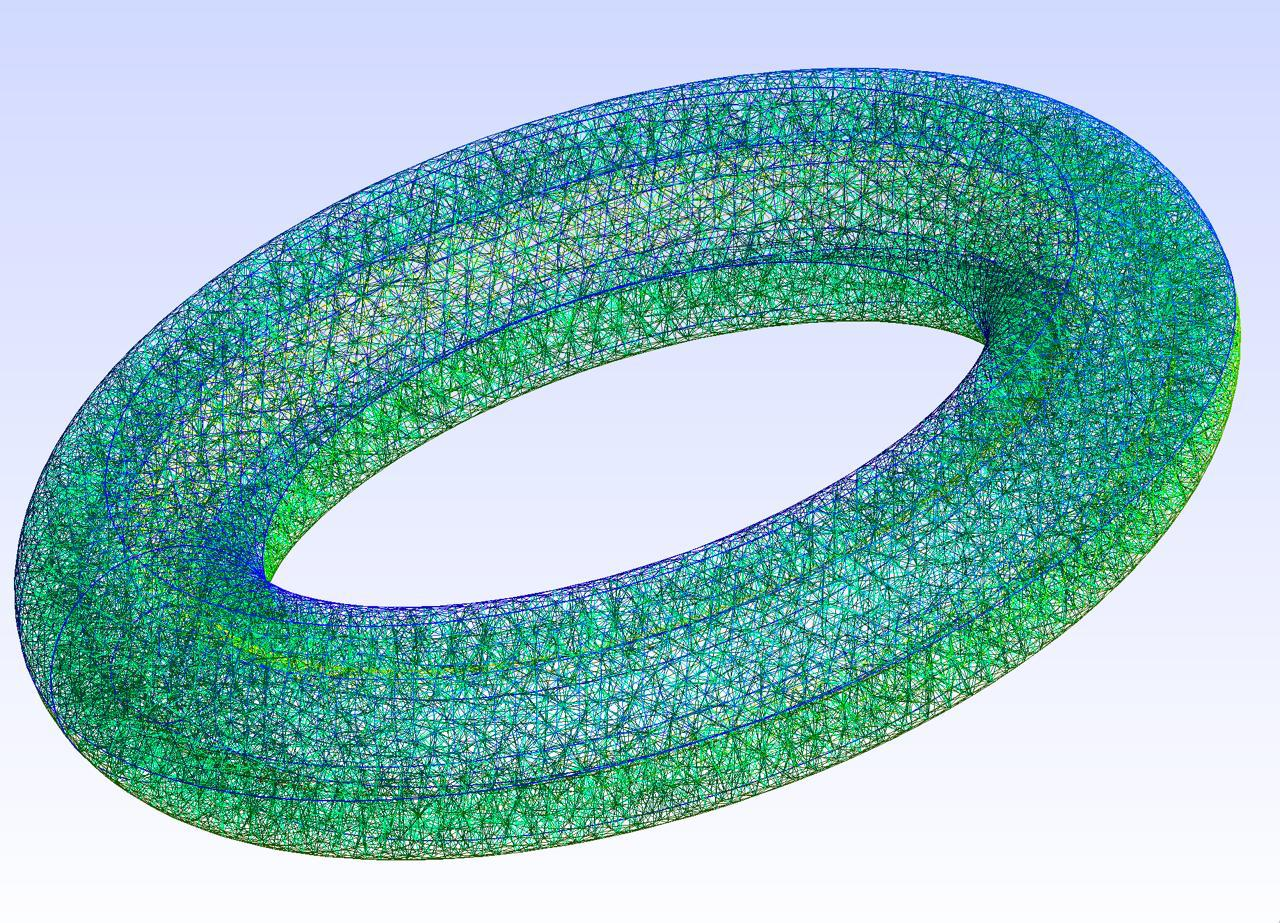
\includegraphics[width=0.75\linewidth]{img/lab1/torus1.png}
  \caption{Тетраэдральная сетка полого тора}
\end{figure}

Вид сбоку показывает, что в толщину стенки укладывается 3--4 элемента,
как и планировалось. Внутри полости элементы вытянутые, но при таком
соотношении размеров этого трудно избежать: радиус $R$ в 4 раза больше
толщины $\Delta r$, и при $h = 0.2$ по окружности получается примерно
20 элементов, а по толщине~--- 3--4.

\begin{figure}[H]
  \centering
  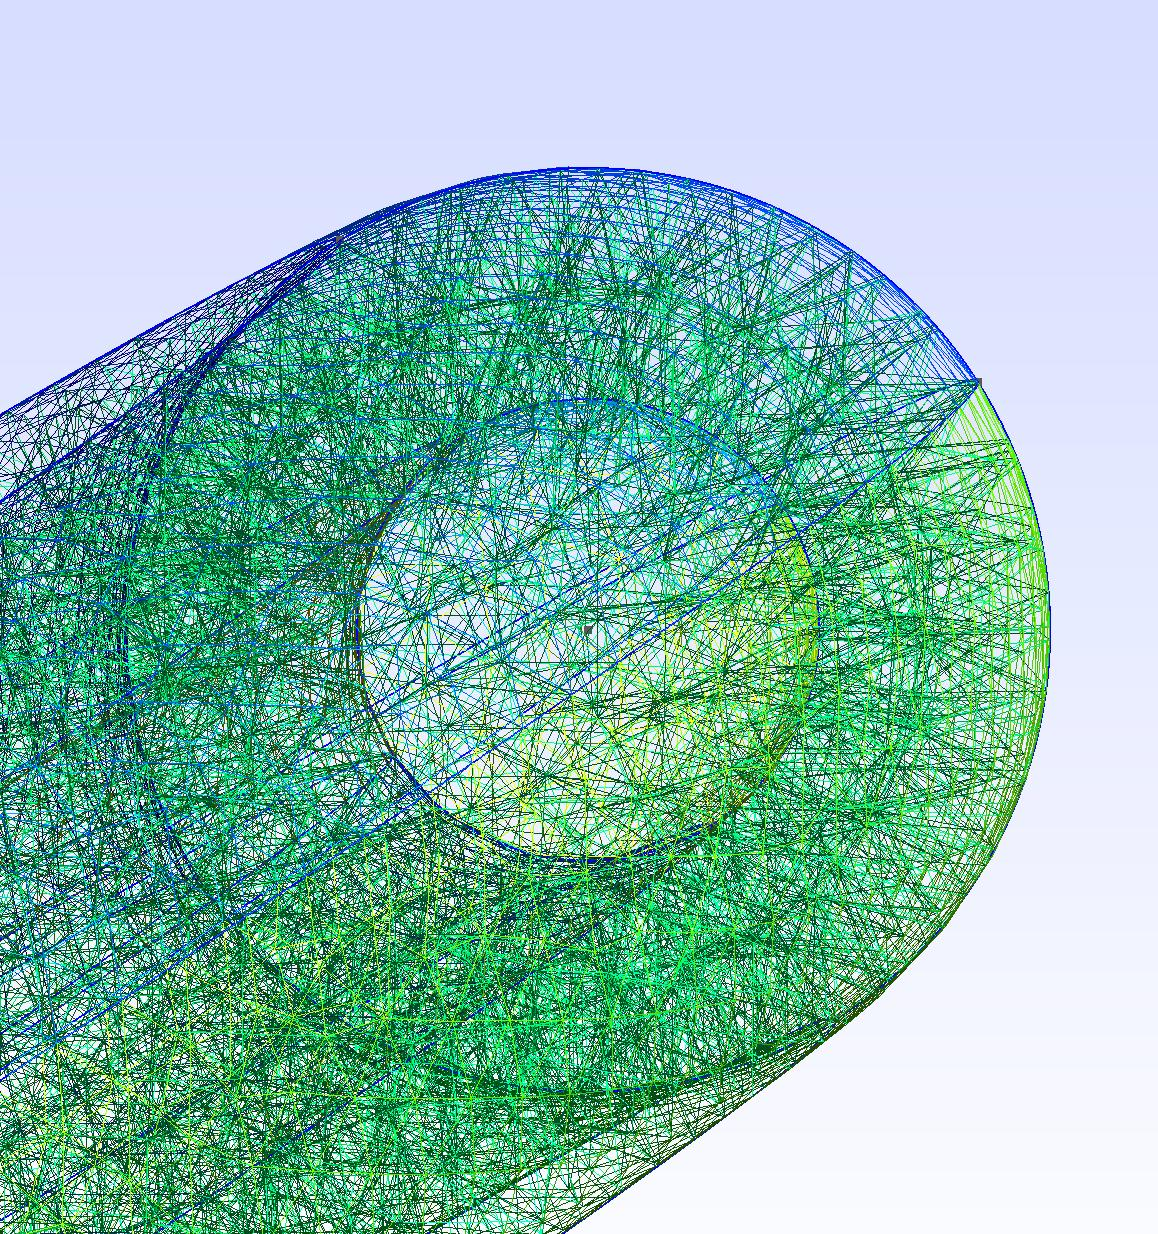
\includegraphics[width=0.5\linewidth]{img/lab1/torus2.png}
  \caption{Тетраэдральная сетка полого тора, вид сбоку}
\end{figure}

\subsection{Этап 2: Сетка в STL-объекте (карандаш)}

\subsubsection{Постановка задачи}

Граница реальных инженерных объектов часто задаётся не аналитически,
а триангулированной поверхностью~--- форматом STL. Это типичный вывод
систем 3D-моделирования и КТ-сканеров. Задача~--- построить объёмную
тетраэдральную сетку \textit{внутри} такого объекта.

\subsubsection{Проблема: STL описывает только поверхность}

STL содержит набор треугольных граней, но не несёт информации об объёме
и не имеет топологии (нет понятия «рёбра», «вершины» в смысле B-Rep).
Чтобы построить объёмную сетку, gmsh должен:
\begin{enumerate}
  \item Классифицировать грани по геометрическим признакам
        (выявить острые рёбра~--- границы патчей);
  \item Параметризовать поверхности~--- задать гладкую геометрию
        каждого патча, пригодную для проецирования узлов сетки;
  \item Сформировать замкнутый объём и заполнить его тетраэдрами.
\end{enumerate}

\subsubsection{Алгоритм классификации поверхностей}

Команда \texttt{classifySurfaces($\alpha$)} разделяет триангуляцию на
патчи: два соседних треугольника относятся к \textit{одному} патчу,
если двугранный угол между ними меньше $\alpha$. Острые рёбра
(угол $\ge \alpha$) становятся границами патчей. Для карандаша
$\alpha = 40^\circ$ отделяет грани ствола от граней заточки и торца.

После классификации \texttt{createGeometry} строит аналитическое
описание каждого патча через B-сплайны~--- это даёт правильные нормали
и возможность точно проецировать узлы на поверхность при генерации сетки.

\subsubsection{Реализация}

\begin{lstlisting}[language=C++, caption={Загрузка STL и построение объёмной сетки}]
gmsh::merge("pencil.stl");
gmsh::model::mesh::classifySurfaces(
    40 * M_PI / 180., true, false, 180 * M_PI / 180.);
gmsh::model::mesh::createGeometry();

vector<pair<int,int>> s;
gmsh::model::getEntities(s, 2);
vector<int> sl;
for (auto surf : s) sl.push_back(surf.second);

int l = gmsh::model::geo::addSurfaceLoop(sl);
gmsh::model::geo::addVolume({l});
gmsh::model::geo::synchronize();

gmsh::option::setNumber("Mesh.CharacteristicLengthMin", 2.0);
gmsh::option::setNumber("Mesh.CharacteristicLengthMax", 2.0);
gmsh::model::mesh::generate(3);
gmsh::write("pencil.msh");
\end{lstlisting}

\subsubsection{Результат}


\begin{figure}[H]
  \centering
  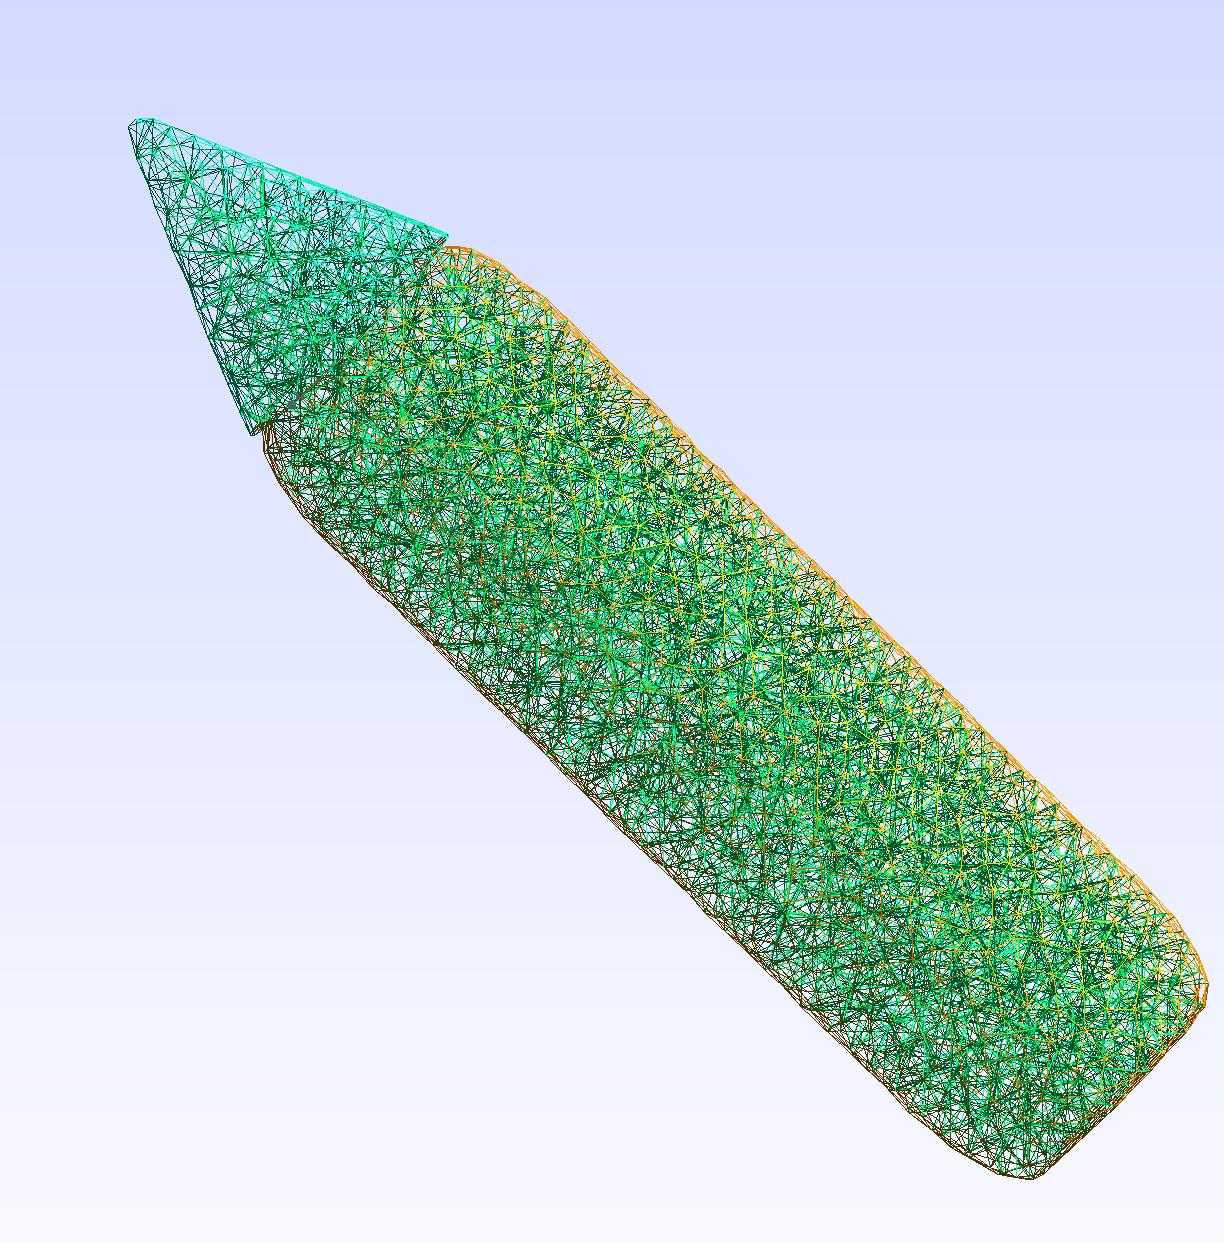
\includegraphics[width=0.75\linewidth]{img/lab1/pencil.png}
  \caption{Тетраэдральная сетка внутри STL-карандаша, $h = 2.0$.}
\end{figure}

\subsection{Выводы}

В работе освоены два принципиально разных подхода к построению
тетраэдральных сеток в gmsh.

\textbf{Конструктивная геометрия (CSG/OCC).} Область задаётся
аналитически~--- через примитивы и булевы операции.

\textbf{Восстановление из STL.} Область задаётся дискретной поверхностью
без аналитического описания. У сложных STL-моделей не всегда получается
автоматически выделить патчи, пригодные для генерации качественной
сетки. В таких случаях модель приходится вручную дорабатывать.

\clearpage

\section{Лабораторная работа \textnumero{}2: ParaView}

\subsection{Цель работы}

Освоить запись результатов расчёта в формат VTK и визуализацию
нестационарных процессов в ParaView на примере распространения
ударной волны в трёхмерной неструктурированной сетке.

\subsection{Постановка задачи}

На сетке из предыдущей лабы (карандаш \texttt{pencil.stl}) моделируется
распространение сферической ударной волны от точечного источника.
В каждом узле сетки на каждом временном шаге вычисляются скалярное
поле давления $p$ и векторное поле скоростей $\mathbf{v}$.

\subsection{Физическая модель}

Волна задаётся аналитически как гауссов импульс, распространяющийся
со скоростью $c$ от точки $(x_0, y_0, z_0)$:
\begin{equation}
  p(\mathbf{x}, t) = v_0
    \exp\!\left(-\frac{(r - ct)^2}{\sigma^2}\right)
    \cdot A(r),
  \qquad r = |\mathbf{x} - \mathbf{x}_0|,
\end{equation}
где затухание $A(r)$ моделирует геометрическое и вязкое рассеяние:
\begin{equation}
  A(r) = \frac{e^{-\alpha r}}{1 + \beta r},
  \quad \alpha = 0.005,\quad \beta = 0.02.
\end{equation}

Отражения от торцов по оси $z$ учитываются зеркальными источниками
с коэффициентом отражения $0.8$ (первый порядок) и $0.64$ (второй порядок).

\subsection{Реализация}

\subsubsection{Загрузка сетки}

Сетка загружается из \texttt{.msh}-файла через gmsh API, узлы и
3D-элементы сохраняются во внутренних структурах \texttt{Node} и
\texttt{Cell}.

\begin{lstlisting}[language=C++, caption={Загрузка узлов из .msh}]
gmsh::model::mesh::getNodes(nodeTags, coords, parametricCoords);
for (size_t i = 0; i < nodeTags.size(); ++i) {
    nodes_[i].x = coords[3*i + 0];
    nodes_[i].y = coords[3*i + 1];
    nodes_[i].z = coords[3*i + 2];
    tag_to_index[nodeTags[i]] = i;
}
\end{lstlisting}

\subsubsection{Временной цикл}

На каждом шаге для каждого узла вычисляется вклад прямой волны
и четырёх зеркальных источников:

\begin{lstlisting}[language=C++, caption={Вычисление поля в узле}]
void PointHit(Node &node, double t) {
    applyWave(hit_center_, node, t, c_, v0_, sigma_);

    Node mirror_top(cx, cy, 2.0*z_max_ - hit_center_.z);
    applyWave(mirror_top,  node, t, c_, v0_*0.8, sigma_);

    Node mirror_bot(cx, cy, 2.0*z_min_ - hit_center_.z);
    applyWave(mirror_bot,  node, t, c_, v0_*0.8, sigma_);
}
\end{lstlisting}

\subsubsection{Запись кадров в VTK}

Каждый кадр записывается в отдельный \texttt{.vtu}-файл:

\begin{lstlisting}[language=C++, caption={Запись кадра в VTK}]
auto grid   = vtkSmartPointer<vtkUnstructuredGrid>::New();
auto smth   = vtkSmartPointer<vtkDoubleArray>::New();
auto vel    = vtkSmartPointer<vtkDoubleArray>::New();
vel->SetNumberOfComponents(3);

for (size_t i = 0; i < nodes_.size(); i++) {
    dumpPoints->InsertNextPoint(nodes_[i].x, nodes_[i].y, nodes_[i].z);
    double v[3] = {nodes_[i].vx, nodes_[i].vy, nodes_[i].vz};
    vel->InsertNextTuple(v);
    smth->InsertNextValue(nodes_[i].smth);
}
string fileName = "pencil-step-" + to_string(snap_number) + ".vtu";
writer->SetFileName(fileName.c_str());
writer->Write();
\end{lstlisting}

\subsection{Параметры расчёта}

\begin{table}[H]
  \centering
  \caption{Параметры расчёта}
  \begin{tabular}{llc}
    \toprule
    Параметр & Описание & Значение \\
    \midrule
    $c$        & Скорость волны            & $15$ ед./с \\
    $v_0$      & Амплитуда                 & $15.0$ \\
    $\sigma$   & Ширина гауссова импульса  & $3.0$ \\
    $\Delta t$ & Шаг по времени            & $0.05$ с \\
    $T$        & Длительность расчёта       & $20.0$ с \\
    $(x_0, y_0, z_0)$ & Источник          & $(2, 0, 85)$ \\
    \bottomrule
  \end{tabular}
\end{table}

\subsection{Визуализация в ParaView}

В ParaView была создана анимация распространения ударной волны внутри
карандаша.

\begin{figure}[H]
  \centering
  
\includegraphics[width=0.8\linewidth]{img/lab2/pencil.png}
  \caption{Кадр из анимации распространения ударной волны.}
\end{figure}

См. \href{https://www.youtube.com/watch?v=DhCUMZFyOzg}{Видео на YouTube}.


\begin{figure}[H]
  \centering
  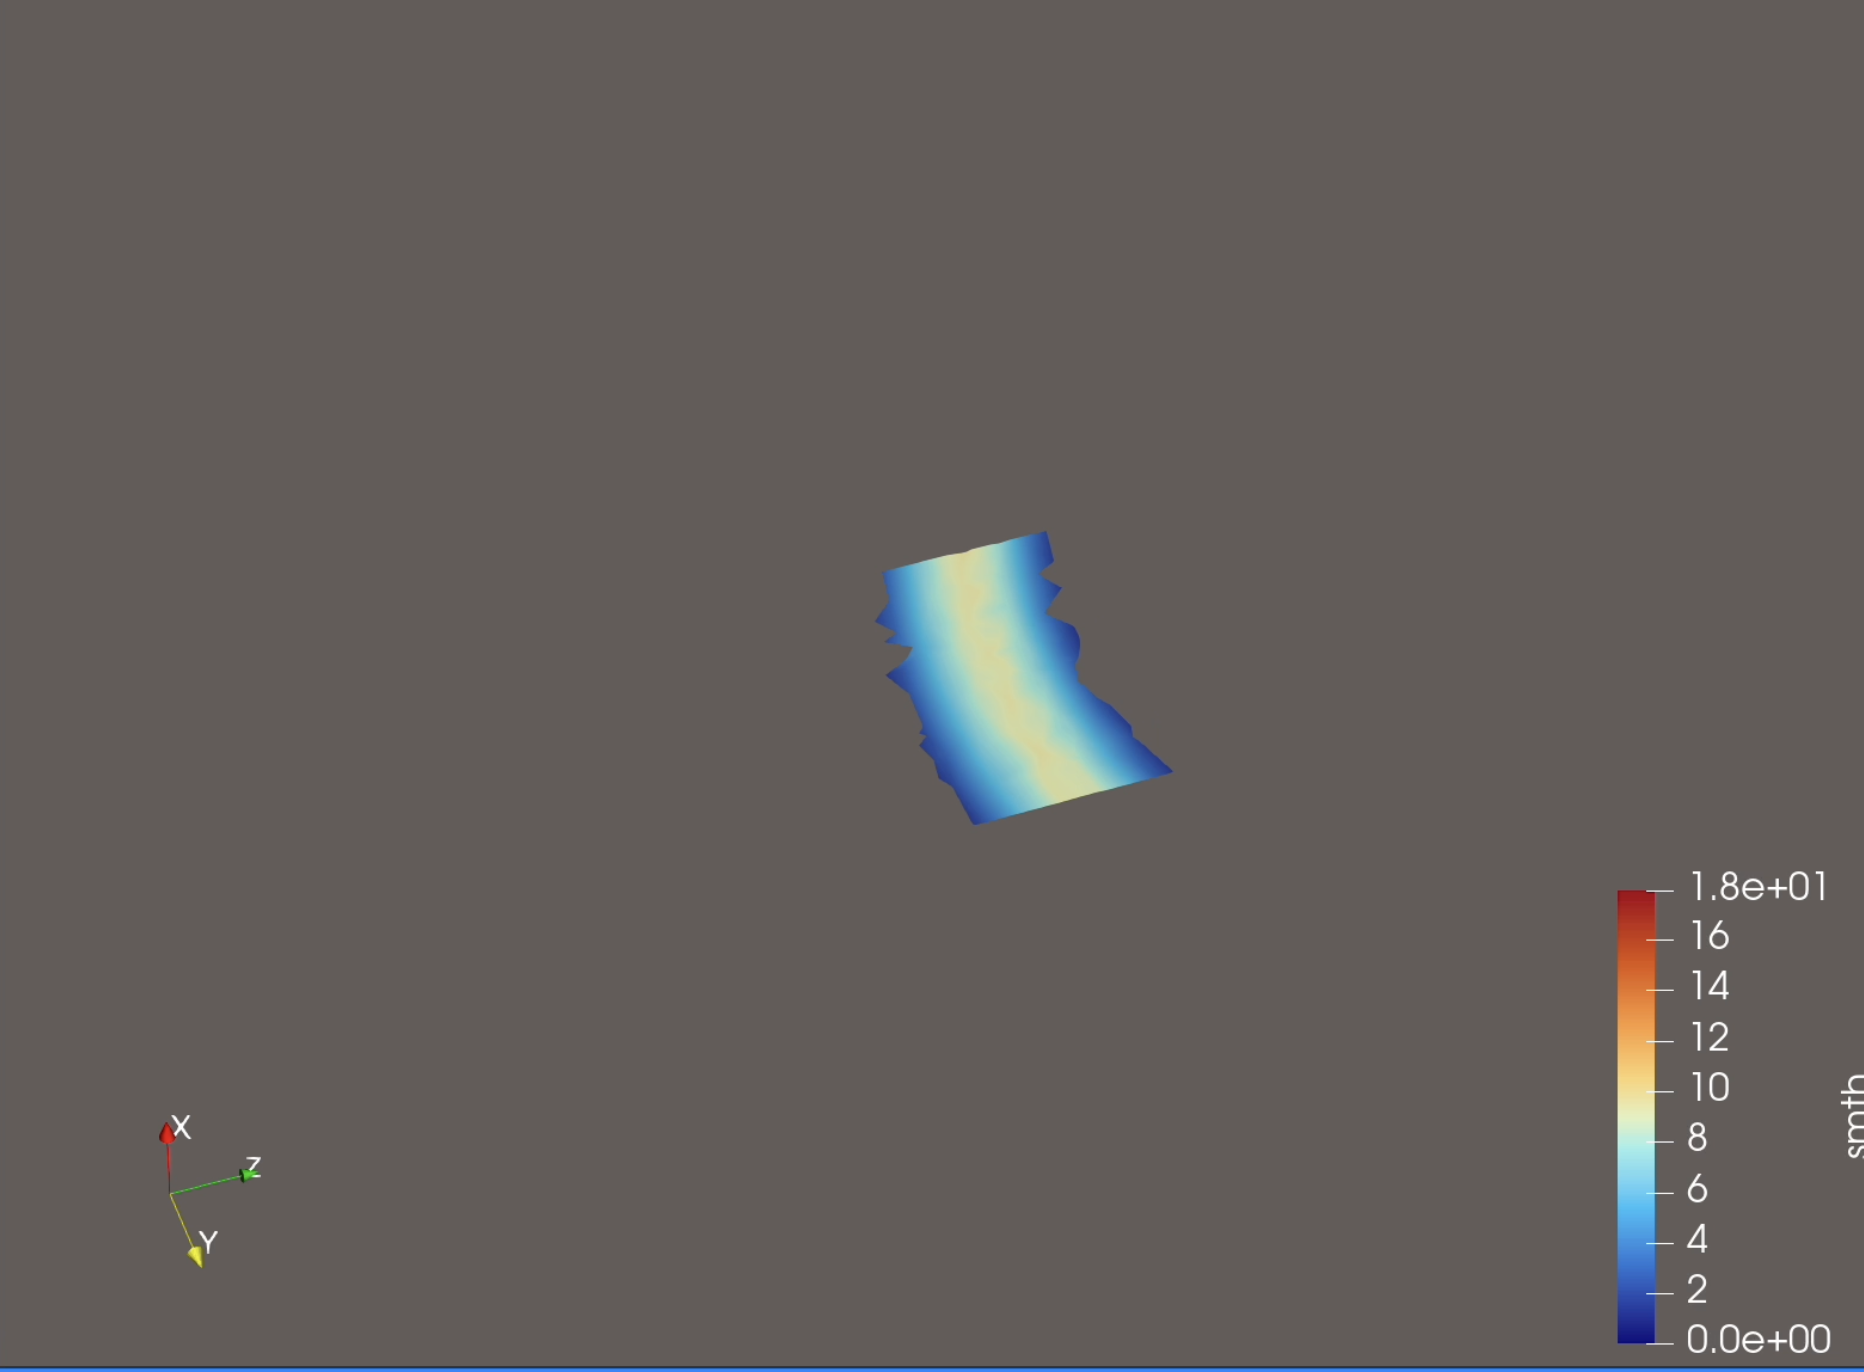
\includegraphics[width=0.8\linewidth]{img/lab2/cut.png}
  \caption{Сечение вдоль оси карандаша с полем ударной волны.}
\end{figure}

\subsection{Выводы}

Реализован цикл расчёта и визуализации нестационарного процесса:
загрузка STL-сетки через gmsh, аналитический расчёт поля волны с учётом
отражений, запись серии \texttt{.vtu}-кадров и визуализация в ParaView.
Использование неструктурированной сетки позволило корректно передать
геометрию объекта произвольной формы.

\clearpage

\section{Лабораторная работа \textnumero{}3: FEniCS}

\subsection{Цель работы}

Научиться ставить эллиптические краевые задачи в FEniCS
и решать их МКЭ. Пример для расчёта~--- электрический диполь
в плоской проводящей среде с локальной неоднородностью.

\subsection{Физическая постановка}

Стационарный потенциал $\phi$ в среде с переменной проводимостью
$\lambda(\mathbf{x})$ подчиняется уравнению:
\begin{equation}\label{eq:strong}
  -\nabla \cdot \bigl(\lambda\,\nabla \phi\bigr) = 0,
  \quad \mathbf{x} \in [-1, 1]^2.
\end{equation}

Электроды~--- малые окружности радиуса $0.1$ с фиксированным потенциалом:
\begin{equation}
  \phi\big|_{\mathbf{x}_+} = +1, \qquad \phi\big|_{\mathbf{x}_-} = -1,
  \qquad \mathbf{x}_\pm = (\pm 0.5,\, 0).
\end{equation}

\subsubsection{Неоднородность среды}

В центре области расположено слабопроводящее гауссово включение:
\begin{equation}\label{eq:lambda}
  \lambda(\mathbf{x}) = \frac{1}{100\,e^{-25\,|\mathbf{x}|^2} + 1}.
\end{equation}
При $|\mathbf{x}| \to 0$ имеем $\lambda \approx 0.01$,
вдали~--- $\lambda \to 1$. Ширина включения~--- $\sigma = 1/\sqrt{25} = 0.2$.

\subsubsection{Слабая формулировка}

Интегрируя по частям, получаем вариационную форму:
\begin{equation}\label{eq:weak}
  \int_\Omega \lambda\,\nabla \phi \cdot \nabla v\,d\mathbf{x} = 0
  \quad \forall\, v \in V_0.
\end{equation}
Неоднородность $\lambda(\mathbf{x})$ входит непосредственно в билинейную
форму, поэтому дополнительных изменений в коде не требуется.

\subsection{Реализация}
Основная часть кода была взята из \href{https://github.com/TheEntityCircle/miniscience-4th-term/tree/master/2025/03_fenics/python}{репозитория} и адаптирована под текущую задачу.

\begin{lstlisting}[language=Python, caption={Сетка, условия Дирихле и решение}]
mesh = RectangleMesh(Point(-1, -1), Point(1, 1), 128, 128)
V    = FunctionSpace(mesh, "Lagrange", 1)

bc_plus  = DirichletBC(V, Constant( 1.0),
    lambda x, _: (x[0]-0.5)**2 + x[1]**2 < 0.01, "pointwise")
bc_minus = DirichletBC(V, Constant(-1.0),
    lambda x, _: (x[0]+0.5)**2 + x[1]**2 < 0.01, "pointwise")

la = Expression("1/(100*exp(-25*(x[0]*x[0]+x[1]*x[1]))+1)", degree=2)

u, v = Function(V), TestFunction(V)
solve(inner(grad(u), grad(v)) * la * dx == 0, u, [bc_plus, bc_minus])
\end{lstlisting}

\begin{lstlisting}[language=Python, caption={Поля E и j через проекцию}]
W = VectorFunctionSpace(mesh, "Lagrange", 1)
E = project(-grad(u),      W)
j = project(-la * grad(u), W)
\end{lstlisting}

Результаты сохранялись в \texttt{.pvd}/\texttt{.vtu} для ParaView.

\subsection{Результаты}
\begin{figure}[H]
  \centering
  
\includegraphics[width=0.8\linewidth]{img/lab3/image.png}
\end{figure}
Вблизи электродов поле имеет ожидаемую диполярную структуру. Линии
тока $\mathbf{j}$ обтекают слабопроводящее включение~--- оно
действует как препятствие, перенаправляя ток в обход центра.

\subsection{Выводы}

Реализовано МКЭ-решение задачи диполя в неоднородной среде.
Картина поля выглядит корректно: ток огибает высокоомное включение.

\clearpage

\part*{II.\quad Микропроект}
\addcontentsline{toc}{part}{II. Микропроект}
\setcounter{section}{0}

\section{Микропроект: задача Стефана (таяние снежинки) (Юрий)}
\subsection{Постановка задачи}

Микропроект посвящён двумерному моделированию фазового перехода лёд--вода
(задача Стефана) энтальпийным методом конечных разностей.
Задача Стефана~--- это задача теплопроводности с подвижной границей:
при плавлении или замерзании граница между фазами перемещается,
поглощая или выделяя скрытую теплоту $L$.

Классическая формулировка требует отслеживания фронта фазового перехода
и выполнения на нём условия Стефана:
\begin{equation}\label{eq:stefan_condition}
  \rho L \frac{ds}{dt} = k_l \frac{\partial T_l}{\partial n}\bigg|_{s}
                       - k_s \frac{\partial T_s}{\partial n}\bigg|_{s},
\end{equation}
где $s(t)$~--- положение фронта, $k_l$, $k_s$~--- теплопроводности жидкой
и твёрдой фаз, $\partial T / \partial n$~--- производные температуры по
нормали к границе с каждой стороны. Это условие выражает баланс тепловых
потоков: разница потоков идёт на плавление (или намерзание) вещества.

В двумерном случае явно отслеживать фронт уже сложно.
Энтальпийный метод позволяет обойти эту проблему, заменяя явное условие
на границе неявной обработкой через функцию $T(H)$.

\subsection{Математическая модель}

\subsubsection{Физические основы}

Рассмотрим среду, состоящую из одного вещества (вода/лёд) с фазовым переходом
I рода при температуре $T_{\rm melt}$. При фазовом переходе I рода
выделяется или поглощается скрытая теплота $L$ (Дж/кг) --- энергия,
необходимая для разрыва межмолекулярных связей кристаллической решётки льда,
не изменяющая при этом температуру вещества.

Теплоперенос в каждой фазе описывается уравнением Фурье:
\begin{equation}\label{eq:fourier}
  \rho c \frac{\partial T}{\partial t} = k\,\nabla^2 T,
\end{equation}
где $\rho$~--- плотность, $c$~--- удельная теплоёмкость, $k$~--- коэффициент
теплопроводности. Это уравнение следует из закона сохранения энергии
и закона Фурье $\mathbf{q} = -k\,\nabla T$, связывающего тепловой поток
с градиентом температуры.

Параметры вещества различаются для твёрдой и жидкой фаз:

\begin{center}
\begin{tabular}{lcc}
  \hline
  Параметр & Лёд & Вода \\
  \hline
  Теплопроводность $k$, Вт/(м$\cdot$К) & 2.2 & 0.6 \\
  Удельная теплоёмкость $c$, Дж/(кг$\cdot$К) & 2090 & 4180 \\
  Скрытая теплота $L$, Дж/кг & \multicolumn{2}{c}{334\,000} \\
  Плотность $\rho$, кг/м$^3$ & \multicolumn{2}{c}{1000} \\
  \hline
\end{tabular}
\end{center}

Температуропроводность $\alpha = k / (\rho c)$ определяет скорость
диффузии тепла: для льда $\alpha_s \approx 1{,}05 \cdot 10^{-6}$~м$^2$/с,
для воды $\alpha_l \approx 1{,}44 \cdot 10^{-7}$~м$^2$/с. Лёд проводит
тепло почти на порядок быстрее воды.

\subsubsection{Энтальпийная формулировка}

Введём объёмную удельную энтальпию $H$ (Дж/м$^3$), отсчитанную от точки
плавления. В этой задаче энтальпия показывает, сколько тепловой энергии
накоплено в единице объёма вещества. Уравнение
теплопроводности в терминах энтальпии принимает единую форму для обеих фаз:
\begin{equation}\label{eq:enthalpy_pde}
  \frac{\partial H}{\partial t} = k\,\nabla^2 T.
\end{equation}

Связь температуры и энтальпии кусочно-линейна:
\begin{equation}\label{eq:T_of_H}
  T(H) = \begin{cases}
    T_{\rm melt} + \dfrac{H}{\rho c_s},          & H < 0          \quad\text{(лёд)}, \\[8pt]
    T_{\rm melt},                                  & 0 \le H \le \rho L \quad\text{(фазовый переход)}, \\[8pt]
    T_{\rm melt} + \dfrac{H - \rho L}{\rho c_l},  & H > \rho L     \quad\text{(вода)}.
  \end{cases}
\end{equation}

Физический смысл трёх областей:
\begin{itemize}
  \item $H < 0$: вещество полностью в твёрдой фазе; вся энергия расходуется
        на изменение температуры;
  \item $0 \le H \le \rho L$: вещество находится в процессе фазового перехода;
        подводимая энергия уходит на фазовый переход, температура при
        этом остаётся равной $T_{\rm melt}$;
  \item $H > \rho L$: вещество полностью в жидкой фазе; вся скрытая теплота
        уже поглощена, дальнейшая энергия снова идёт на нагрев.
\end{itemize}

Ключевое достоинство энтальпийного метода: граница раздела фаз
обрабатывается автоматически. Ячейки, в которых $0 \le H \le \rho L$,
находятся <<в процессе>> фазового перехода~--- фронт плавления
распределяется по нескольким ячейкам сетки, не требуя явного
отслеживания его положения.

\subsubsection{Теплопроводность в зоне фазового перехода}

В ячейках, находящихся в процессе плавления ($0 \le H \le \rho L$),
теплопроводность интерполируется между фазами:
\begin{equation}
  k(H) = (1 - f)\,k_s + f\,k_l, \qquad f = \frac{H}{\rho L},
\end{equation}
где $f \in [0,1]$~--- доля жидкой фазы. Это обеспечивает плавный
переход теплофизических свойств через фронт.

\subsection{Численный метод}

\subsubsection{Явная конечно-разностная схема}

Уравнение~(10) дискретизируется на равномерной
квадратной сетке $N \times N$ с шагом $h = D / N$, где $D$~--- размер
области. Лапласиан аппроксимируется стандартным пятиточечным шаблоном:
\begin{equation}\label{eq:scheme}
  H_{i,j}^{n+1} = H_{i,j}^{n}
    + \Delta t \cdot k_{i,j}
    \cdot \frac{T_{i+1,j}^n + T_{i-1,j}^n + T_{i,j+1}^n + T_{i,j-1}^n
          - 4\,T_{i,j}^n}{h^2},
\end{equation}
где $k_{i,j} = k(H_{i,j}^n)$~--- теплопроводность, зависящая от фазы.

Схема является \textbf{явной}: значения на новом временном слое $n+1$
вычисляются непосредственно из значений на слое $n$, без решения
системы линейных уравнений. Это даёт простую реализацию, но накладывает
ограничение на шаг по времени.

\subsubsection{Условие устойчивости}

Явная схема устойчива при выполнении условия CFL:
\begin{equation}\label{eq:cfl}
  \Delta t \le \frac{h^2\,\rho\,c_{\min}}{4\,k_{\max}},
\end{equation}
где множитель 4 соответствует двумерному случаю (четыре соседа в шаблоне),
$c_{\min}$ и $k_{\max}$~--- наименьшая теплоёмкость и наибольшая
теплопроводность среди фаз. Физический смысл: за один шаг по времени
тепло не должно <<перескочить>> через ячейку.

Для используемых параметров ($h = 10^{-4}$~м, $k_{\max} = 2{,}2$,
$c_{\min} = 2090$, $\rho = 1000$):
\[
  \Delta t_{\max} \approx 2{,}4 \cdot 10^{-3}~\text{с}.
\]

\subsubsection{Граничные условия}

Реализованы два типа граничных условий:

\textbf{Фиксированные (Дирихле):}
температура на границе не меняется~--- $T|_{\partial\Omega} = T_0$.
Используется для моделирования контакта с телом заданной температуры
(например, рука при $36\,^{\circ}$C).

\textbf{Адиабатические (Нейман):}
тепловой поток через границу равен нулю~---
$\partial T / \partial n|_{\partial\Omega} = 0$.
Реализуется копированием энтальпии из ближайшей внутренней ячейки.
Используется для замкнутых систем без теплообмена с окружением.

\subsubsection{Двойная буферизация}

При обновлении сетки по схеме~(13) значения $T_{i\pm1,j}^n$
и $T_{i,j\pm1}^n$ должны быть со \textit{старого} временного слоя.
Поэтому используется буфер $H_{\rm new}$: сначала все новые значения
записываются в буфер, затем буфер копируется обратно в основной массив.

\subsection{Валидация}

\subsubsection{Одномерная задача Стефана}

Для верификации численной схемы рассмотрена одномерная задача: полупространство
льда при $T = T_{\rm melt}$, левая граница мгновенно нагревается до $T_{\rm hot}$.
Аналитическое решение даёт положение фронта плавления:
\begin{equation}\label{eq:stefan_exact}
  s(t) = 2\lambda\sqrt{\alpha_l\, t},
\end{equation}
где $\alpha_l = k_l / (\rho c_l)$~--- температуропроводность жидкой фазы,
а $\lambda$~--- корень трансцендентного уравнения:
\begin{equation}\label{eq:transcendental}
  \mathrm{St} = \lambda\sqrt{\pi}\,e^{\lambda^2}\,\mathrm{erf}(\lambda),
\end{equation}
где $\mathrm{St} = c_l (T_{\rm hot} - T_{\rm melt}) / L$~--- число Стефана,
характеризующее отношение теплоты, затраченной на нагрев жидкости,
к скрытой теплоте плавления. При $T_{\rm hot} = 50\,^{\circ}$C:
\[
  \mathrm{St} = \frac{4180 \cdot 50}{334\,000} \approx 0{,}626.
\]

\begin{figure}[H]
  \centering
  
\includegraphics[width=1.00\linewidth]{img/micro/validation.png}
  \caption{Сравнение численного положения фронта $s(t)$ с аналитическим
           решением. Численный фронт
           воспроизводит закон $s \propto \sqrt{t}$.}
\end{figure}

\subsection{Постановки задач (сцены)}

\subsubsection{Таяние снежинки}

Снежинка задаётся PNG-маской: тёмные пиксели маски инициализируются как лёд
($H = \rho c_s \cdot (T_0 - T_{\rm melt}) < 0$), окружающая среда~--- как
тёплая вода ($H = \rho L + \rho c_l \cdot (T_w - T_{\rm melt}) > \rho L$).
Тонкие лучи тают первыми, так как у них наибольшее отношение поверхности
к объёму: тепло проникает к центру тонкого элемента быстрее.

\subsubsection{Таяние снежинки на руке}

Снежинка помещается на нижнюю границу области с фиксированной температурой
$T_{\rm hand} = 36\,^{\circ}$C (температура тела человека). Окружающий воздух
моделируется как лёд при $T \approx 0\,^{\circ}$C. При размере снежинки $\sim 5$~мм
и реальных теплофизических параметрах время полного таяния составляет 2--3~с,
что качественно совпадает с повседневным опытом.

\subsubsection{Намерзание (сосулька)}

Вода при $+2\,^{\circ}$C, верхняя стенка охлаждена до $-20\,^{\circ}$C,
боковые стенки при $+5\,^{\circ}$C. Лёд нарастает сверху вниз; тёплые
боковые границы не дают ему расшириться, формируя вытянутую структуру.
Эта постановка демонстрирует обратимость фазового перехода: тот же
солвер без изменений моделирует и плавление, и замерзание.

\subsection{Реализация}

\subsubsection{Архитектура}

Проект реализован на C++17 с разделением на модули:
\begin{itemize}
  \item \texttt{core/}~--- физика (Grid, Solver, Material). Не зависит от
        библиотеки визуализации;
  \item \texttt{render/}~--- визуализация (Renderer, Colormap). Зависит
        от raylib, не знает о деталях физики;
  \item \texttt{scenes/}~--- начальные условия. Каждая сцена реализует
        интерфейс \texttt{Scene};
  \item \texttt{export/}~--- вывод данных в CSV для анализа в Python.
\end{itemize}

Зависимости однонаправлены: \texttt{render} $\to$ \texttt{core} (только чтение),
\texttt{scenes} $\to$ \texttt{core}. Циклических зависимостей нет.

\subsubsection{Оптимизация рендеринга}

Наивная отрисовка $N \times N$ прямоугольников через \texttt{DrawRectangle}
($\sim 40\,000$ вызовов при $N = 200$) даёт $\sim 4$~FPS. Вместо этого
температурное поле записывается в массив пикселей, загружается как текстура
на GPU (\texttt{UpdateTexture}) и отрисовывается одним вызовом
\texttt{DrawTextureEx}. Результат: $\sim 60$~FPS.

\subsubsection{Интерактивное управление}

Raylib-приложение поддерживает:
\begin{itemize}
  \item \texttt{[1]--[5]}~--- переключение сцен;
  \item \texttt{[SPACE]}~--- пауза / продолжение;
  \item \texttt{[R]}~--- сброс состояния;
  \item \texttt{[LMB]}~--- локальный нагрев мышью;
  \item \texttt{[RMB]}~--- локальное охлаждение мышью;
  \item \texttt{[F]}~--- запись кадров в PNG.
\end{itemize}

\subsection{Результаты}



\begin{figure}[H]
  \centering
  
\includegraphics[width=0.8\linewidth]{img/micro/image.png}
    \caption{Таяние снежинки. Синий~--- лёд, белый~--- фазовый переход,
           красный~--- вода. Тонкие лучи исчезают первыми.}
\end{figure}

См. \href{https://www.youtube.com/watch?v=3Jm9fgB6ytE&feature=youtu.be}{Видео на YouTube}.

Качественные наблюдения:
\begin{enumerate}
  \item Тонкие элементы снежинки тают быстрее массивных~--- следствие
        большего отношения площади поверхности к объёму.
  \item Фронт плавления в 1D воспроизводит аналитический закон
        $s \propto \sqrt{t}$.
  \item Намерзание и плавление обрабатываются одним и тем же кодом без
        изменений~--- обратимость фазового перехода I рода.
\end{enumerate}

\subsection{Выводы}

Реализован двумерный решатель задачи Стефана энтальпийным методом
на явной конечно-разностной схеме. Энтальпийная формулировка позволяет
избежать явного отслеживания фронта плавления, сохраняя физически
корректную картину фазового перехода. Валидация на одномерном
аналитическом решении подтвердила корректность реализации.

Продемонстрированы три режима: таяние (снежинка в тёплой воде),
контактное плавление (снежинка на руке) и намерзание (рост льда
от холодного источника). Все режимы обрабатываются единым солвером
без изменения уравнений~--- это следствие энтальпийной
формулировки.

\clearpage

\section{Микропроект 2: ультразвуковой импульс в 3D-модели головы (Артём)}
\subsection{Постановка задачи}

Второй микропроект посвящён моделированию распространения короткого
ультразвукового импульса в трёхмерной анатомической модели головы.
Искомая величина~--- акустическое давление $p(\mathbf{x}, t)$,
распространяющееся по неоднородной среде: мягким тканям, костям,
кровеносным сосудам и другим областям, заданным на тетраэдральной сетке.

Цель работы~--- собрать полный расчётный пайплайн:
\begin{enumerate}
  \item взять готовую сегментированную 3D-модель головы;
  \item перенести материал каждой ячейки в DOLFINx;
  \item задать импульсный ультразвуковой источник;
  \item решить нестационарную акустическую задачу методом конечных элементов;
  \item сохранить результаты в формате \texttt{.vtu} для ParaView.
\end{enumerate}

Геометрическая модель взята из репозитория
\href{https://github.com/avasyukov/gcm-3d/tree/markered-corpse/models/ani3d}{gcm-3d},
ветка с моделями \texttt{ani3d}. Это готовая тетраэдральная сетка
анатомической области с метками материалов. Расчётный код был написан
с опорой на готовые примеры из
\href{https://github.com/adeebkor/fenicsx-fus}{fenicsx-fus}, где уже
используется DOLFINx для задач ультразвука.

\subsection{Расчётная модель}

\subsubsection{Геометрия и материалы}

В каталоге \texttt{mini\_project/3d-models/} используются два основных
VTU-файла:
\begin{itemize}
  \item \texttt{mesh.vtu}~--- исходная неструктурированная тетраэдральная
        сетка головы;
  \item \texttt{head\_with\_materials.vtu}~--- сетка после предобработки,
        где к каждой ячейке добавлены поля \texttt{material\_id},
        \texttt{rho}, \texttt{lambda}, \texttt{mu},
        \texttt{sound\_speed}.
\end{itemize}
В итоговой сетке:
\[
  N_{\rm points}=125\,215, \qquad N_{\rm cells}=729\,468.
\]

Координаты модели используются в миллиметрах, время~--- в секундах,
поэтому скорость звука в коде задаётся в мм/с. Плотность и упругие
константы берутся из таблицы материалов, приведённой в том же источнике,
что и модель.

\begin{center}
\begin{tabular}{lcccc}
  \hline
  Область & Material ID & $\rho$, г/мм$^3$ & $c$, мм/с
          & $(\lambda, \mu)$ \\
  \hline
  Жир & 3, 31 & $1{,}158\cdot 10^{-3}$ & $1{,}45\cdot 10^6$
      & $(3{,}07\cdot 10^6,\;2{,}05\cdot 10^6)$ \\
  Мышцы / мягкие ткани & 4, 11, 12, 27, 30, 32
      & $1{,}00\cdot 10^{-3}$ & $1{,}58\cdot 10^6$
      & $(3{,}07\cdot 10^6,\;2{,}05\cdot 10^6)$ \\
  Кость & 21 & $1{,}00\cdot 10^{-3}$ & $3{,}50\cdot 10^6$
      & $(7{,}86\cdot 10^8,\;1{,}18\cdot 10^9)$ \\
  Кровь & 22, 28, 29 & $1{,}00\cdot 10^{-3}$ & $1{,}57\cdot 10^6$
      & $(2{,}39\cdot 10^5,\;5{,}00\cdot 10^2)$ \\
  Трахея & 24 & $2{,}00\cdot 10^{-3}$ & $1{,}54\cdot 10^6$
      & $(1{,}43\cdot 10^7,\;3{,}57\cdot 10^6)$ \\
  Аорта & 25 & $1{,}00\cdot 10^{-3}$ & $1{,}57\cdot 10^6$
      & $(9{,}21\cdot 10^6,\;1{,}90\cdot 10^5)$ \\
  Вены & 26 & $1{,}00\cdot 10^{-3}$ & $1{,}57\cdot 10^6$
      & $(3{,}289\cdot 10^7,\;6{,}70\cdot 10^5)$ \\
  \hline
\end{tabular}
\end{center}

В акустической постановке непосредственно используются $\rho(\mathbf{x})$
и $c(\mathbf{x})$. Константы Ламе $\lambda(\mathbf{x})$, $\mu(\mathbf{x})$
сохранены в модели для следующего шага~--- линейно-упругого расчёта
смещений.

\subsubsection{Предобработка сетки}

Файл \texttt{preprocess.py} читает VTU через \texttt{meshio}, находит
тетраэдральный блок и восстанавливает \texttt{Material ID} для каждой
ячейки.

Материалы записываются в ячейки:
\begin{equation}
  \rho_h,\; c_h,\; \lambda_h,\; \mu_h \in DG_0(\Omega),
\end{equation}
то есть каждое значение постоянно внутри одного тетраэдра.

\subsection{Физическая постановка}

\subsubsection{Линейная акустика}

Ультразвуковой импульс рассматривается как малая добавка давления
к равновесному состоянию среды. Поэтому используется линейная акустика:
амплитуда возмущения мала по сравнению с модулем объёмного сжатия,
а нелинейные эффекты и поглощение в первом приближении не учитываются.

Пусть $\mathbf{v}(\mathbf{x},t)$~--- акустическая скорость частиц среды,
$p(\mathbf{x},t)$~--- акустическое давление, $\rho(\mathbf{x})$~---
плотность, $c(\mathbf{x})$~--- скорость звука. Для малых возмущений:
\begin{equation}
  \rho(\mathbf{x})\,\frac{\partial \mathbf{v}}{\partial t}
  = -\nabla p,
\end{equation}
\begin{equation}
  \frac{1}{\rho(\mathbf{x})c^2(\mathbf{x})}
  \frac{\partial p}{\partial t}
  + \nabla\cdot\mathbf{v} = 0.
\end{equation}
Первое уравнение~--- линеаризованный закон Ньютона: градиент давления
разгоняет частицы среды. Второе~--- связь сжимаемости и давления:
при сжатии объёма давление растёт; коэффициент
$K=\rho c^2$ играет роль объёмного модуля.

Исключая $\mathbf{v}$, получаем волновое уравнение в неоднородной среде:
\begin{equation}\label{eq:acoustic_strong}
  \frac{1}{\rho(\mathbf{x})c^2(\mathbf{x})}
  \frac{\partial^2 p}{\partial t^2}
  - \nabla\cdot\left(
      \frac{1}{\rho(\mathbf{x})}\nabla p
    \right)
  = s(\mathbf{x},t).
\end{equation}

Если $\rho$ и $c$ постоянны, оно сводится к обычному уравнению
$p_{tt}-c^2\Delta p = \rho c^2 s$. В данной задаче коэффициенты
кусочно-постоянны по тканям, поэтому фронт волны меняет скорость,
отражается и преломляется на границах материалов.

\subsubsection{Источник}

Источник разделён на пространственную и временную части:
\begin{equation}
  s(\mathbf{x},t)=g(\mathbf{x})\,q(t).
\end{equation}

Пространственный профиль~--- гауссово пятно:
\begin{equation}
  g(\mathbf{x}) =
  A \exp\left(
    -\frac{\|\mathbf{x}-\mathbf{x}_s\|^2}{2\sigma^2}
  \right).
\end{equation}
В коде центр $\mathbf{x}_s$ ставится около нижней границы расчётной
области:
\begin{equation}
  x_s=\frac{x_{\min}+x_{\max}}{2}, \qquad
  y_s=y_{\min}+0{,}4(y_{\max}-y_{\min}), \qquad
  z_s=z_{\min},
\end{equation}
а ширина берётся как $\sigma=0{,}1\,D$, где $D$~--- максимальный
габаритный размер модели.

Временная форма~--- короткий ультразвуковой пакет с плавным окном:
\begin{equation}\label{eq:burst}
q(t)=
\begin{cases}
  \sin(2\pi f\tau)\,
  \sin^2\left(\dfrac{\pi\tau}{T}\right),
  & 0 \le \tau \le T,\\[8pt]
  0, & \text{иначе},
\end{cases}
\end{equation}
где
\[
  \tau=t-t_{\rm start}, \qquad
  t_{\rm start}=t_0-\frac{T}{2}, \qquad
  T=\frac{N}{f}.
\]

В расчёте:
\[
  f = 1~\text{МГц}, \qquad N=5, \qquad
  t_0=\frac{5}{f}, \qquad T=\frac{5}{f}.
\]
Множитель $\sin^2(\pi\tau/T)$ плавно поднимает амплитуду от нуля и
возвращает её обратно к нулю. Это уменьшает артефакты, которые появились
бы при резком обрыве синуса.

\subsubsection{Граничные условия}

Явно заданных граничных условий Дирихле в акустическом коде нет.
После интегрирования по частям естественное граничное условие имеет вид
\begin{equation}
  \left.
  \frac{1}{\rho}\nabla p\cdot\mathbf{n}
  \right|_{\partial\Omega}=0.
\end{equation}
Физически это отражающая граница.

\subsection{Численный метод}

\subsubsection{Слабая формулировка}

Умножим уравнение~\eqref{eq:acoustic_strong} на тестовую функцию
$v \in V$ и проинтегрируем по области. С учётом естественного
граничного условия получаем:
\begin{equation}\label{eq:acoustic_weak}
  \int_\Omega
  \frac{1}{\rho c^2}\,
  \frac{\partial^2 p}{\partial t^2}\,v\,d\mathbf{x}
  +
  \int_\Omega
  \frac{1}{\rho}\,\nabla p\cdot\nabla v\,d\mathbf{x}
  =
  q(t)\int_\Omega g(\mathbf{x})v\,d\mathbf{x}.
\end{equation}

Используется пространство конечных элементов Лагранжа первой степени
на тетраэдральной сетке:
\[
  V_h = \{v_h:\; v_h|_K \in P_1(K)\}.
\]


\subsubsection{Полудискретная система}

После FEM-дискретизации получаем систему ОДУ:
\begin{equation}\label{eq:semi_discrete}
  \mathbf{M}\ddot{\mathbf{p}} + \mathbf{K}\mathbf{p}
  = q(t)\mathbf{F},
\end{equation}
где
\begin{equation}
  M_{ij} = \int_\Omega
  \frac{1}{\rho c^2}\,\phi_i\phi_j\,d\mathbf{x},
\end{equation}
\begin{equation}
  K_{ij} = \int_\Omega
  \frac{1}{\rho}\,\nabla\phi_j\cdot\nabla\phi_i\,d\mathbf{x},
\end{equation}
\begin{equation}
  F_i = \int_\Omega g(\mathbf{x})\phi_i\,d\mathbf{x}.
\end{equation}

Матрица жёсткости $\mathbf{K}$ собирается обычным образом через
\texttt{assemble\_matrix}. Для матрицы масс используется диагональное
приближение: вместо полной матрицы хранится вектор сумм по строкам.
Так явный шаг становится дешевле: не нужно решать линейную систему на
каждом временном слое.

\subsubsection{Явная схема по времени}

Для второй производной по времени используется центральная разность:
\begin{equation}
  \ddot{\mathbf{p}}^n \approx
  \frac{\mathbf{p}^{n+1}-2\mathbf{p}^{n}+\mathbf{p}^{n-1}}{\Delta t^2}.
\end{equation}
Подставляя это в~\eqref{eq:semi_discrete}, получаем явную схему:
\begin{equation}\label{eq:explicit_acoustic}
  \mathbf{p}^{n+1}
  =
  2\mathbf{p}^{n}-\mathbf{p}^{n-1}
  +
  \Delta t^2\,\mathbf{M}_L^{-1}
  \left(
    q(t_n)\mathbf{F}-\mathbf{K}\mathbf{p}^{n}
  \right).
\end{equation}

Начальные условия нулевые:
\[
  p(\mathbf{x},0)=0, \qquad
  \frac{\partial p}{\partial t}(\mathbf{x},0)=0.
\]

\subsubsection{Условие устойчивости}

Явная схема для волнового уравнения требует шага, согласованного
со скоростью распространения волны и минимальным размером элемента.
В коде шаг оценивается автоматически:
\begin{equation}
  \Delta t =
  \mathrm{safety}\,
  \frac{h_{\min}}{c_{\max}},
  \qquad
  \mathrm{safety}=0{,}25.
\end{equation}
Здесь $h_{\min}$ вычисляется через \texttt{cpp.mesh.h}.
\[
  c_{\max}=3{,}5\cdot 10^6~\text{мм/с}.
\]

\subsection{Реализация}

\subsubsection{Структура проекта}

Основные файлы:
\begin{itemize}
  \item \texttt{mini\_project/src/acoustic\_impulse.py}~--- основной
        акустический расчёт;
  \item \texttt{mini\_project/src/tools/preprocess.py}~--- загрузка VTU,
        перенос \texttt{Material ID}, создание DG0-полей;
  \item \texttt{mini\_project/src/tools/convert\_to\_vtu\_with\_materials.py}~---
        добавление физических параметров в VTU-файл;
\end{itemize}

Результаты пишутся в папку
\texttt{mini\_project/src/acoustic\_vtu\_frames\_other\_source/}
как последовательность \texttt{.vtu}-кадров.

\subsubsection{Контроль устойчивости}

Если шаг времени или амплитуда источника выбраны неправильно, решение
быстро начинает неограниченно расти, и расчёт останавливается.

Дополнительно задан порог
\[
  \max |p| \le 10^6 \text{Па}.
\]
Если давление превышает этот предел, программа сообщает, на каком шаге
произошла ошибка и останавливается.

\subsection{Результаты}

При запуске акустического расчёта импульс рождается около верхней границы
головы и распространяется через неоднородную анатомическую структуру.
Из-за различий в $c(\mathbf{x})$ и $\rho(\mathbf{x})$ фронт не остаётся
сферическим: на границах тканей возникают отражения и изменения длины
волны. Особенно заметное влияние дают костные области, где скорость
звука больше, чем в мягких тканях.

\begin{figure}[H]
  \centering
  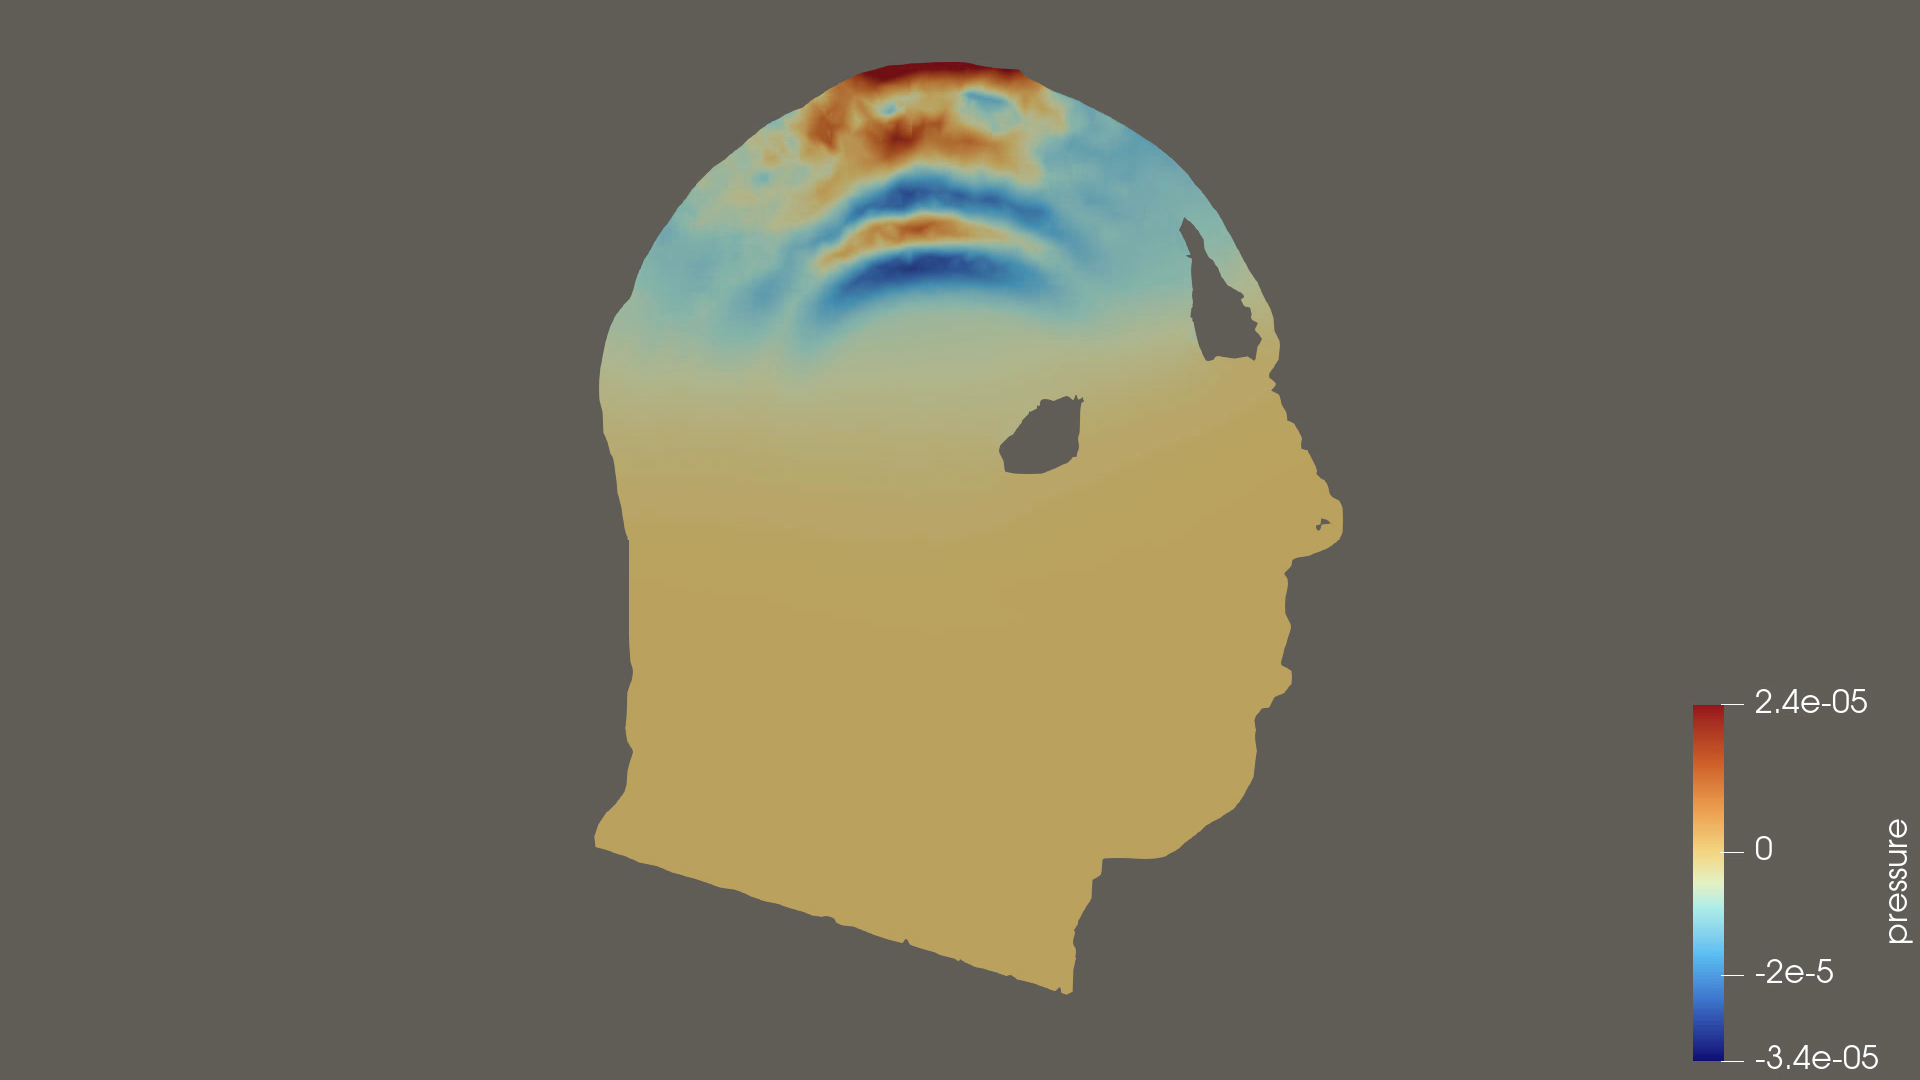
\includegraphics[width=0.78\linewidth]{micro2/acoustic_impulse.png}
  \caption{Кадр визуализации акустического давления в ParaView.
           Красно-синие области соответствуют положительным и отрицательным
           фазам ультразвукового импульса.}
\end{figure}

По результатам расчёта были получены VTU-кадры и видеовизуализации.
См. \href{https://disk.360.yandex.ru/d/l9_8UlurSN1kMA}{примеры видео на Яндекс Диске}.

\subsection{Выводы}

В работе собран рабочий FEM-пайплайн для моделирования ультразвукового
импульса в 3D-модели головы. Главный результат~--- переход от готовой
анатомической VTU-сетки к физической DOLFINx-модели: метки материалов
сохранены, коэффициенты $\rho$ и $c$ назначены, а давление
рассчитано явной схемой на тетраэдральной сетке.

Физическая постановка соответствует линейной акустике в неоднородной
среде. Использование импульсного источника даёт короткий
ультразвуковой сигнал.

\clearpage

\part*{III.\quad Макропроект}
\addcontentsline{toc}{part}{III. Макропроект}
\setcounter{section}{0}

\section{Макропроект: тепловой блок задачи LSP}
\subsection{Постановка задачи}

Макропроект~--- первая ступень в цепочке моделей лазерной ударной
проковки (LSP): короткий лазерный импульс нагревает поверхность металла,
вызывая быстрое локальное расширение; ударная волна создаёт в объёме
зону остаточных сжимающих напряжений, повышая усталостную прочность.

Цепочка из трёх блоков:
\begin{enumerate}
  \item \textbf{Тепловой (наш):} лазерный импульс $\to$ поле $T(\mathbf{r},t)$
        с учётом плавления.
  \item \textbf{Конвертер:} $T, f_l \to$ термоупругий источник
        (член Дюгамеля--Неймана).
  \item \textbf{Механический (напарник):} распространение упругих волн
        в образце.
\end{enumerate}

В рамках макропроекта реализованы первый блок и интерфейс ко второму:
3D-обобщение энтальпийного солвера, лазерный источник как граничное
условие Неймана, замена среды на алюминий, экспорт в VTK для прямой
передачи в механический код.

\subsection{Физическая постановка}

\subsubsection{Геометрия и масштабы}

Тонкая пластина алюминия $2 \times 2 \times 0{,}05$~мм. Лазер падает
нормально на верхнюю грань, гауссово пятно радиуса $r_L = 0{,}5$~мм
(на уровне $1/e^2$). Боковые и нижняя грани~--- теплоизолированы:
глубина прогрева за время импульса $\sqrt{\chi\tau} \sim 1$~мкм $\ll L_z$.

Импульс~--- гауссиан по времени, FWHM $\tau = 10$~нс, пиковая интенсивность
$I_0 = 10^{12}$~Вт/м$^2$~--- режим прямого нагрева без абляции.

\subsubsection{Уравнение энергии}

Энтальпийная формулировка в 3D:
\begin{equation}
  \frac{\partial H}{\partial t}
  = \nabla \cdot \bigl( k(T)\,\nabla T \bigr) + Q(\mathbf{r}, t).
\end{equation}
Кусочно-линейная связь $T(H)$ и интерполяция $k$ через долю жидкой
фазы переносятся из микропроекта без изменений. Опорная температура
$T_{\rm ref} = 300$~К: $H = 0$ соответствует холодному твёрдому
материалу.

\subsubsection{Материал}

\begin{center}
\begin{tabular}{lcc}
  \hline
  Параметр & Твёрдый Al & Жидкий Al \\
  \hline
  $k$, Вт/(м$\cdot$К) & 237 & 91 \\
  $c$, Дж/(кг$\cdot$К) & 900 & 1180 \\
  $T_{\rm melt}$, К & \multicolumn{2}{c}{933} \\
  $L$, Дж/кг & \multicolumn{2}{c}{$3{,}97 \cdot 10^{5}$} \\
  $\rho$, кг/м$^3$ & \multicolumn{2}{c}{2700} \\
  \hline
\end{tabular}
\end{center}

Температуропроводность $\chi_s \approx 10^{-4}$~м$^2$/с~--- на два
порядка выше, чем у льда. Это определяет на три порядка меньший шаг
по времени по сравнению с микропроектом.

\subsubsection{Источник лазера}

Поглощённый поток на верхней грани:
\begin{equation}
  q_{\rm abs}(x, y, t) = (1 - R)\, I_0\,
    \exp\!\left(-\frac{(t - t_0)^2}{2\sigma_t^2}\right)
    \exp\!\left(-\frac{2\bigl((x-x_c)^2+(y-y_c)^2\bigr)}{r_L^2}\right).
\end{equation}

Длина оптического проникновения в металл $\delta \sim 10$~нм мельче
шага сетки, поэтому объёмное тепловыделение заменяется эквивалентным
граничным условием Неймана на верхней грани.

\subsection{Численный метод}

\subsubsection{Дивергентная схема}

В микропроекте лапласиан аппроксимировался через $k\nabla^2 T$
с теплопроводностью в центре ячейки. На полке плавления $k$ меняется,
и такая форма нарушает локальный энергобаланс.

В макропроекте схема переписана в дивергентной форме. Поток через грань
между ячейками $i$ и $i+1$:
\begin{equation}
  F_{i+1/2} = -k_{i+1/2}\, \frac{T_{i+1} - T_i}{\Delta x},
  \qquad
  k_{i+1/2} = \frac{2\, k_i\, k_{i+1}}{k_i + k_{i+1}}.
\end{equation}
Гармоническое среднее~--- стандарт для последовательно соединённых
слоёв. Поток, вышедший из ячейки, точно равен потоку, вошедшему в
соседнюю~--- баланс энергии выполняется на уровне дискретизации.

\subsubsection{Устойчивость}

CFL в 3D с семиточечным шаблоном:
\begin{equation}
  \Delta t \le \frac{\Delta h_{\min}^2}{6\,\chi_{\max}}.
\end{equation}
При сетке $64 \times 64 \times 32$ ($\Delta z \approx 1{,}6$~мкм)
получается $\Delta t_{\max} \sim 4 \cdot 10^{-10}$~с; с запасом $0{,}4$
берётся $\Delta t \approx 1{,}7 \cdot 10^{-10}$~с. Весь импульс
$200$~нс~--- $\sim 1200$ шагов.

\subsubsection{Граничные условия}

Все грани, кроме верхней,~--- адиабат (зеркальное копирование энтальпии).
Верхняя грань: вместо потока через несуществующую внешнюю грань
подставляется $-q_{\rm abs}(x_i, y_j, t^n)$.

\subsection{Реализация}

\subsubsection{Архитектура}

Raylib и сцены из микропроекта удалены. Структура:
\begin{itemize}
  \item \texttt{core/}~--- \texttt{Grid}, \texttt{Solver},
        \texttt{SimMaterial}. Headless, без внешних зависимостей.
  \item \texttt{scenes/}~--- единственная сцена \texttt{LaserPulse}:
        однородный старт $T = 300$~К, $q_{\rm abs}$ на верхней грани.
  \item \texttt{export/}~--- \texttt{VtkWriter} (VTU + временная серия
        \texttt{.pvd}), \texttt{ProbeWriter} (CSV-зонд в центре пятна).
\end{itemize}

Сборка~--- один вызов CMake без \texttt{find\_package}.

\subsubsection{Экспорт}

Декартова сетка переупаковывается в неструктурированную тетраэдрическую:
каждая ячейка бьётся на 5 тетраэдров без вспомогательных узлов
(тип VTK\_TETRA). В каждом кадре:
\begin{itemize}
  \item \texttt{PointData}: $T$, $H$, \texttt{liquid\_fraction},
        \texttt{phase};
  \item \texttt{FieldData}: 13 материальных констант (теплофизика,
        оптика, механика)~--- напарник читает их из того же файла.
\end{itemize}
Один кадр ($131\,072$ узла, $615\,195$ тетраэдра)~--- $\approx 17$~МБ.

Стыковка проверена: минимальный тестовый \texttt{.vtu} прочитан
пайплайном напарника в ParaView и через dolfinx.

\subsection{Результаты}

При $I_0 = 10^{12}$~Вт/м$^2$, $\tau = 10$~нс, $R = 0{,}3$ температура
в центре пятна поднимается с $300$~К до $\approx 1000$~К за $\sim 30$~нс,
после чего выходит на полку $T_{\rm melt} = 933$~К: дальнейшая энергия
уходит в скрытую теплоту. Зона $f_l > 0$~--- приповерхностный слой
глубиной несколько микрометров.

Грубая энергетическая оценка даёт глубину расплава $\sim 1$~мкм~---
согласуется с расчётом.

Полный прогон~--- ${\sim}20$~с на одном ядре; 100 кадров VTU~---
${\sim}1{,}7$~ГБ, основное узкое место.

\begin{figure}[H]
  \centering
  
\includegraphics[width=0.8\linewidth]{img/macro/image.png}
    \caption{Таяние снежинки. Синий~--- лёд, белый~--- фазовый переход,
           красный~--- вода. Тонкие лучи исчезают первыми.}
\end{figure}
См. \href{https://youtu.be/QrDzDw7RYcw}{Видео на YouTube}.

\subsection{Направления развития}

\begin{enumerate}
  \item \textbf{Термоупругий пересчёт.}
        $\varepsilon^{\rm therm} = 3\alpha_T(T - T_0) + (\Delta V/V)\,f_l$~---
        второе слагаемое даёт вклад от фазового перехода, ради которого
        и нужен полный энтальпийный расчёт.

  \item \textbf{Абляция (формула Fabbro).} При $I_0 > 10^{13}$~Вт/м$^2$
        доминирует плазменное давление; подаётся в механический код
        отдельно как Neumann-BC на поверхности.

  \item \textbf{Произвольная геометрия.} Сейчас~--- параллелепипед.
        Минимальная переделка~--- маска «внутри/снаружи» поверх
        декартовой сетки.

  \item \textbf{JSON-конфиг.} Параметры сцены сейчас в \texttt{main.cpp};
        вынести в файл, читаемый обоими кодами.
\end{enumerate}

\subsection{Выводы}

Реализован 3D тепловой блок для задачи LSP на основе энтальпийного
метода. Ключевые изменения относительно 2D-микропроекта: дивергентная
форма потоков с гармоническим усреднением $k$ (точный энергобаланс),
замена среды на алюминий, лазерный источник как Neumann-ГУ, экспорт
в тетраэдрический VTU с временной серией.

Физическая картина~--- глубина и размер зоны плавления~--- согласуется
с энергетическими оценками. Интерфейс с механическим блоком проверен;
полная цепочка LSP становится возможной после реализации термоупругого
пересчёта на стороне напарника.
\clearpage

% ============================================================
%  bibliography.tex -- список литературы
% ============================================================

\addcontentsline{toc}{section}{Список литературы}

\begin{thebibliography}{9}

\bibitem{abramowitz}
  Абрамовиц М., Стиган И.
  \textit{Справочник по специальным функциям.}
  Наука, 1979.

\bibitem{vtk}
  Schroeder W., Martin K., Lorensen B.
  \textit{The Visualization Toolkit.}
  Kitware, 4th ed., 2006.

\bibitem{fenics}
  Logg A., Mardal K.-A., Wells G.
  \textit{Automated Solution of Differential Equations by the Finite Element Method.}
  Springer, 2012.

% TODO: добавить нужные источники

\end{thebibliography}


\end{document}
